\documentclass[a4paper, final]{article}
%\usepackage{literat} % Нормальные шрифты
\usepackage[14pt]{extsizes} % для того чтобы задать нестандартный 14-ый размер шрифта
\usepackage[T2A]{fontenc}
\usepackage[UTF8]{inputenc}
\usepackage[english]{babel}
\usepackage{listings} %листинги
\usepackage{amsmath}
\usepackage{amssymb} % Для красивого значка пустого множества
\usepackage[left=25mm, top=20mm, right=20mm, bottom=20mm, footskip=10mm]{geometry}
\usepackage{ragged2e} %для растягивания по ширине
\usepackage{setspace} %для межстрочного интервала
\usepackage{indentfirst} % для абзацного отступа
\usepackage{moreverb} %для печати в листинге исходного кода программ
\renewcommand\verbatimtabsize{4\relax}
\renewcommand\listingoffset{0.2em} %отступ от номеров строк в листинге
\renewcommand{\arraystretch}{1.4} % изменяю высоту строки в таблице
\usepackage[font=small, singlelinecheck=false, justification=centering, format=plain, labelsep=period]{caption} %для настройки заголовка таблицы
\usepackage{listingsutf8}
\usepackage{xcolor} % цвета
\usepackage{hyperref}% для гиперссылок
\usepackage{enumitem} %для перечислений
\usepackage{titlesec}
\usepackage{graphicx}
\graphicspath{ {./Рисунки/} }
%\usepackage{float}
\usepackage{booktabs}
\usepackage{floatrow}
\usepackage{scalerel} % Stretching images
\usepackage[final]{pdfpages}
\usepackage{multirow}
\usepackage{array}
\usepackage{tabularx}
\usepackage{caption} % заголовки плавающих объектов

\captionsetup[figure]{name=Fig} % заголовок рисунков
\captionsetup[table]{name=Table} % заголовок рисунков

\definecolor{apricot}{HTML}{FFF0DA}
\definecolor{mygreen}{rgb}{0,0.6,0}
\definecolor{string}{HTML}{B40000} % цвет строк в коде
\definecolor{comment}{HTML}{008000} % цвет комментариев в коде
\definecolor{keyword}{HTML}{1A00FF} % цвет ключевых слов в коде
\definecolor{morecomment}{HTML}{8000FF} % цвет include и других элементов в коде
\definecolor{captiontext}{HTML}{FFFFFF} % цвет текста заголовка в коде
\definecolor{captionbk}{HTML}{999999} % цвет фона заголовка в коде
\definecolor{bk}{HTML}{FFFFFF} % цвет фона в коде
\definecolor{frame}{HTML}{999999} % цвет рамки в коде
\definecolor{brackets}{HTML}{B40000} % цвет скобок в коде





\AtBeginDocument{\renewcommand{\contentsname}{Contents}}
\AtBeginDocument{\renewcommand{\refname}{References}}
% Настраиваем листинги, чтобы они использовали счётчик figure
\AtBeginDocument{
  \renewcommand{\thelstlisting}{\thefigure}  % Листинги используют тот же счетчик, что и рисунки
  \renewcommand{\lstlistingname}{Fig.}    % Меняем подпись
}

% Автоматически увеличиваем счетчик figure перед каждым листингом
\let\oldlstlisting\lstlisting
\renewcommand{\lstlisting}[1][]{%
    \refstepcounter{figure}% Увеличиваем счетчик figure
    \oldlstlisting[#1]% Вызываем оригинальную команду lstlisting
}
\lstset{
    captionpos=b
}
\newcommand{\specialcell}[2][l]{\begin{tabular}[#1]{@{}l@{}}#2\end{tabular}} % Алиас для таблиц

\floatsetup[table]{style=plain,capposition=top} % Подпись таблицы сверху
\setlist[enumerate,itemize]{leftmargin=1.2cm} %отступ в перечислениях

\hypersetup{colorlinks,
  allcolors=[RGB]{010 090 200}} %красивые гиперссылки (не красные)

% подгружаемые языки — подробнее в документации listings (это всё для листингов)
\lstloadlanguages{ [LaTeX] TeX}
% включаем кириллицу и добавляем кое−какие опции
\lstset{language =[LaTeX] TeX, % выбираем язык по умолчанию
extendedchars=true , % включаем не латиницу
escapechar = | , % |«выпадаем» в LATEX|
frame=tb , % рамка сверху и снизу
commentstyle=\itshape , % шрифт для комментариев
stringstyle =\bfseries} % шрифт для строк

\textheight=24cm % высота текста
\textwidth=16cm % ширина текста
\oddsidemargin=0pt % отступ от левого края
\topmargin=-1.5cm % отступ от верхнего края
\parindent=24pt % абзацный отступ
\parskip=0pt % интервал между абзацами
\tolerance=2000 % терпимость к ``жидким`` строкам
\flushbottom % выравнивание высоты страниц

\begin{document} % начало документа
\setcounter{tocdepth}{2} % Вложенность не больше 2 в содержании
% НАЧАЛО ТИТУЛЬНОГО ЛИСТА
\begin{center}
    \hfill \break
    \hfill \break
    \normalsize{MINISTRY OF SCIENCE AND HIGHER EDUCATION OF THE RUSSIAN FEDERATION\\
    Federal State Autonomous Educational Institution of Higher Education Peter the Great St. Petersburg Polytechnic University\\[10pt]}
    \normalsize{Institute of Computer Science and Cybersecurity}\\[10pt] 
    \normalsize{Higher School of Artificial Intelligence Technology}\\[10pt] 
    \normalsize{Direction 02.03.01 Mathematics and computer Science}\\
    
    \hfill \break
    \hfill \break
    \hfill \break
    \hfill \break
    \large{\textbf{Literature Review}}\\
    \large{\textit{Workflow Scheduling Algorithms for High-Performance Computing and Cloud Environments}}\\
    
    \hfill \break
    \hfill \break
\end{center}

\small{ 
    \begin{tabular}{lrrl}
        \!\!\!Student, & \hspace{2cm} & & \\
        \!\!\!group 5130201/20102 & \hspace{2cm} & \underline{\hspace{3cm}} & Gaar V. S. \\\\
        \!\!\!Supervisor, Ph. D. & \hspace{2cm} &  \underline{\hspace{3cm}} &  Motorin D. E. \\\\
        &&\hspace{4cm}
    \end{tabular}
    \begin{flushright}
        <<\underline{\hspace{1cm}}>>\underline{\hspace{2.5cm}} 2024г.
    \end{flushright}
}

\hfill \break
% \hfill \break
\begin{center} \small{Saint-Petersburg, 2024} \end{center}
\thispagestyle{empty} % выключаем отображение номера для этой страницы

% КОНЕЦ ТИТУЛЬНОГО ЛИСТА
\newpage

\tableofcontents

\cleardoublepage
\phantomsection
\newpage
\addcontentsline{toc}{section}{Abstract}
\section*{Abstract}
Workflow scheduling is critical in optimizing the performance of high-performance computing (HPC) and 
cloud environments, where efficient resource allocation and task execution are paramount. This literature 
review provides a comprehensive comparative analysis of ten advanced workflow scheduling algorithms developed 
for various computing environments, including HPC, mobile edge computing (MEC), cloud computing, and hybrid systems. 
The methodologies are examined concerning their mathematical foundations, optimization techniques, application domains, 
and adaptability to dynamic workloads and system scalability. Performance outcomes are analyzed based on execution time 
optimization, energy efficiency, cost reduction, privacy preservation, and resource utilization. The review identifies 
common strengths such as adaptability and multi-objective optimization, while also highlighting key differences and 
trade-offs in addressing conflicting objectives. Limitations are discussed, and future research directions are proposed, 
including the integration of renewable energy sources, enhanced privacy mechanisms, and the exploration of hybrid 
optimization techniques. The findings underscore the significant role of advanced scheduling algorithms in improving 
system performance and resource management in HPC and cloud environments.

\cleardoublepage
\phantomsection
\newpage
\addcontentsline{toc}{section}{Keywords}
\section*{Keywords}
Workflow Scheduling, High-Performance Computing (HPC), Mobile Edge Computing (MEC), Cloud Computing, 
Directed Acyclic Graph (DAG), Resource Allocation, Data Privacy, Optimization Algorithms, 
Energy Efficiency, Latency Reduction.

\newpage
\cleardoublepage
\phantomsection
\section{Introduction}
Workflow scheduling plays a pivotal role in modern computing environments, where the complexity and scale of tasks have 
grown exponentially. These environments include High-Performance Computing (HPC) \cite{bib:1_acrl}, Mobile Edge 
Computing (MEC) \cite{bib:2_faro}, \cite{bib:6_marine}, Edge Function as a Service (Edge FaaS) \cite{bib:4_faas}, 
Geographically Distributed Cloud Data Centers (GD-CDCs) \cite{bib:5_epee}, \cite{bib:7_ppps}, and hybrid cloud-edge 
ecosystems \cite{bib:8}, \cite{bib:9}, each characterized by unique challenges and requirements. The surge in data-intensive 
applications -- ranging from artificial intelligence workloads to real-time IoT systems -- has amplified the demand for 
efficient scheduling mechanisms that can dynamically allocate resources, optimize execution time, and minimize energy 
consumption while adhering to evolving privacy regulations.

The advent of distributed systems introduces complexities that traditional scheduling methods struggle to address. 
Distributed computing environments are inherently heterogeneous, involving diverse resource types such as CPUs, GPUs, 
memory, and network bandwidth, which must be coordinated to meet the demands of complex workflows. A 
common representation of such workflows is through a Directed Acyclic Graph (DAG), as shown in Fig.~\ref{fig:1} of  \cite{bib:1_acrl}, 
where nodes represent tasks, and edges define dependencies. Moreover, the dynamic nature of workloads, where task 
priorities and resource availability fluctuate unpredictably, exacerbates the need 
for adaptable and resilient scheduling mechanisms \cite{bib:3_sandcat}. Additionally, these systems often span 
multiple geographic regions, as seen in GD-CDCs and hybrid cloud models, where data transfer costs, latency, and 
privacy constraints further complicate resource allocation \cite{bib:7_ppps}, \cite{bib:9}.

\begin{figure}[H]
   \centering
   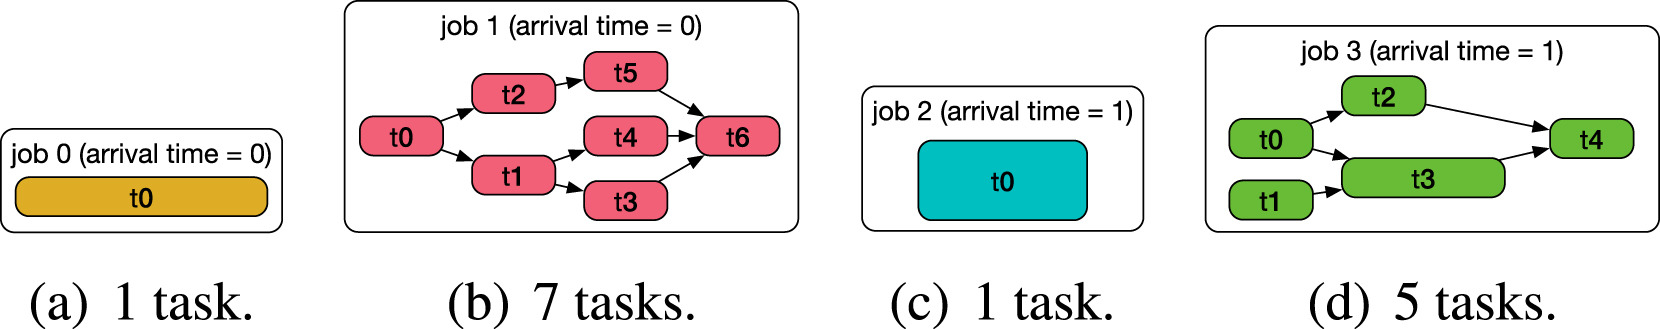
\includegraphics[scale=1.5]{dag.jpg}
   \caption{Examples of tasks and jobs with distinct arrival times and demands (in terms of processing and expected 
   walltime). Each rectangle represents a task: processing is denoted by the rectangle height and execution time by 
   the base’s length. The arrows represent the execution’s workflow.}
   \label{fig:1}
\end{figure}

Energy efficiency has emerged as a critical consideration, particularly in edge and cloud computing environments, 
where power consumption directly impacts operational costs and sustainability goals. Studies such as
exploration of DVFS-based optimization \cite{bib:5_epee} highlight the growing emphasis on energy-aware scheduling, 
which seeks to balance resource utilization with energy savings. Similarly, edge-focused systems like those addressed 
in \cite{bib:3_sandcat} aim to optimize energy consumption while ensuring low latency, which is 
critical for real-time applications such as autonomous vehicles and industrial IoT.

Another dimension of complexity lies in the integration of data privacy requirements, particularly in geo-distributed 
systems. As workflows increasingly operate across multiple jurisdictions, privacy-preserving mechanisms, such as those 
proposed in \cite{bib:7_ppps}, are essential to comply with regional data protection laws, reflected in the Fig.~\ref{fig:privacy}
of \cite{bib:7_ppps} while maintaining operational efficiency. These privacy constraints introduce new trade-offs between WAN usage, data 
locality, and computational overhead, necessitating innovative approaches to graph partitioning and workflow 
scheduling \cite{bib:8}.

\begin{figure}[H]
   \centering
   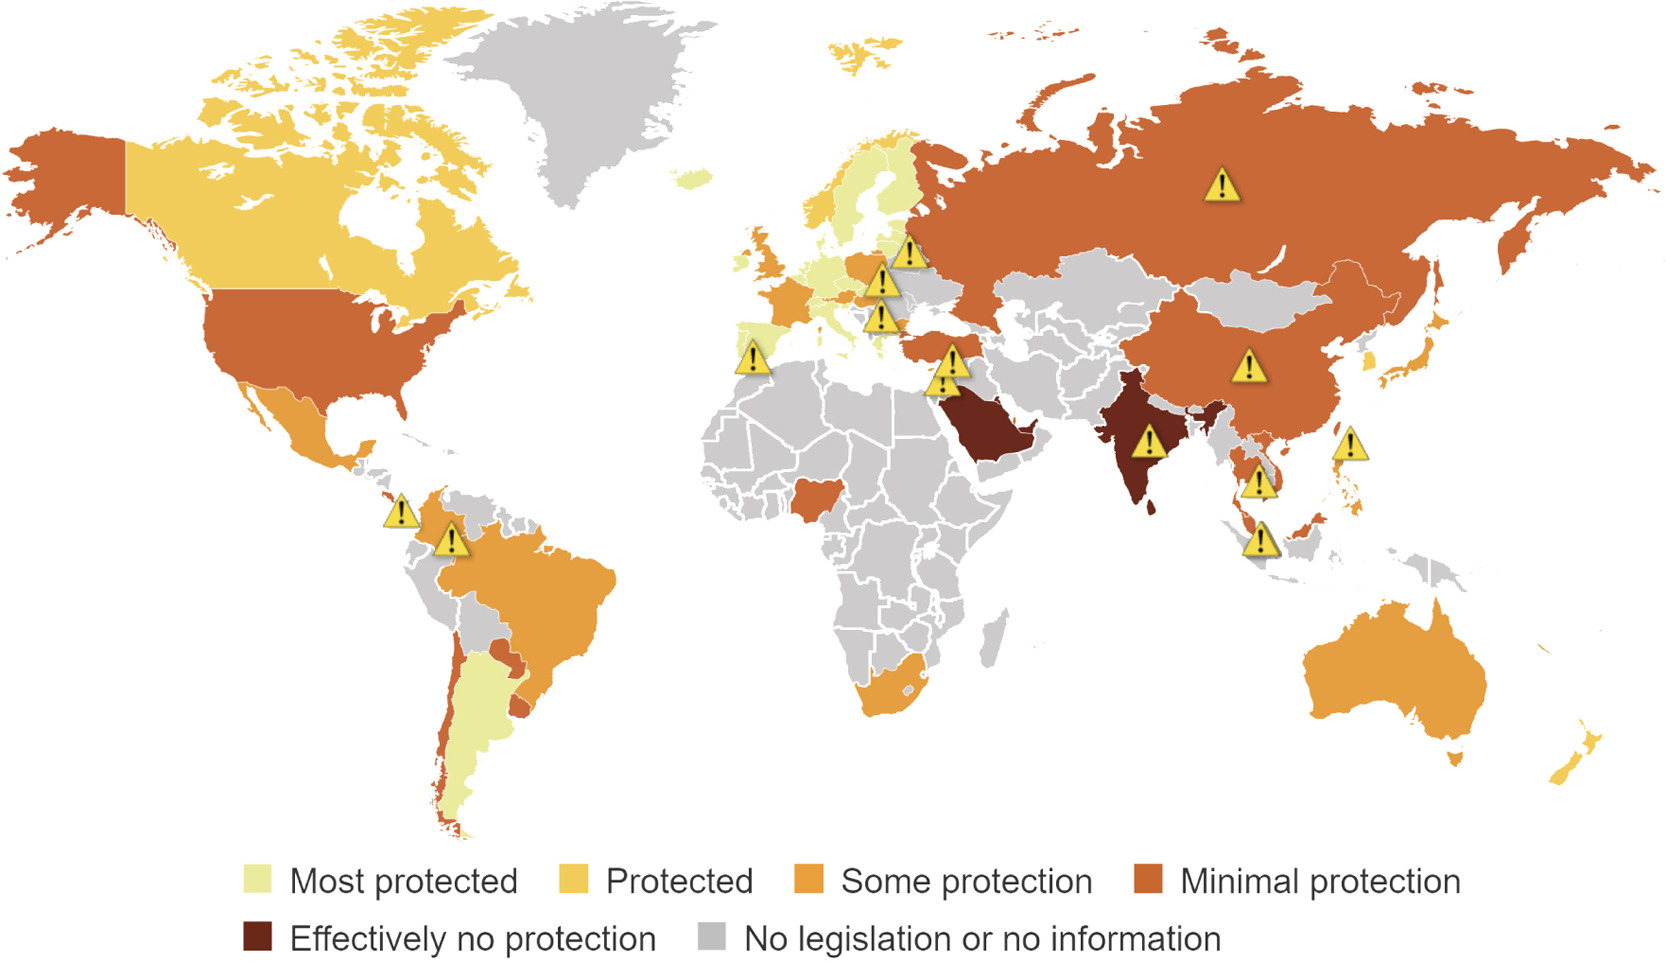
\includegraphics[scale=1.5]{privacy.jpg}
   \caption{A comparative ranking of 54 countries’ privacy and data protection requirements.}
   \label{fig:privacy}
\end{figure}

The core challenges shared across all ten reviewed studies include:

\begin{itemize}
\item Efficient resource allocation in heterogeneous environments, ensuring fair distribution of computational resources 
such as CPU, memory, and network bandwidth.
\item Dynamic task scheduling to adapt to unpredictable workloads and fluctuating resource availability in real time.
\item Optimization of key performance metrics, such as execution time, cost, energy consumption, and latency, to achieve 
global system efficiency.
\item Scalability and flexibility, enabling systems to handle growing workloads and infrastructure expansions without 
significant performance degradation.
\item Integration of privacy and regulatory constraints, particularly in systems spanning multiple regions with varying 
legal requirements \cite{bib:7_ppps}, \cite{bib:10}.
\end{itemize}

To address these challenges, researchers have turned to machine learning, heuristic and metaheuristic optimization 
algorithms, and hybrid approaches that combine static and dynamic scheduling strategies. Examples include the use of 
Actor-Critic Reinforcement Learning \cite{bib:1_acrl}, multi-strategy heuristic optimization \cite{bib:3_sandcat}, and 
genetically modified particle swarm optimization \cite{bib:10}. These methods represent a shift towards more adaptable, 
intelligent scheduling frameworks that balance multiple objectives simultaneously.

This literature review focuses on the comparative analysis of these innovative scheduling approaches, highlighting 
their strengths, limitations, and potential for integration into future systems. The studies collectively advance the 
field by addressing the pressing need for scalable, energy-efficient, and privacy-compliant workflow scheduling, 
offering insights into how these methods can be adapted for the evolving landscape of distributed computing.

The review is structured as follows: Section 2 provides background and context, discussing the 
significance of workflow scheduling, the challenges faced, and the evolution from traditional to 
advanced algorithms. Section 3 presents a comparative analysis of the scheduling methods, including a 
detailed examination of their mathematical and programming approaches, optimization techniques, 
application domains, and adaptability. Section 4 analyzes and compares the performance outcomes of the 
algorithms based on key metrics. Section 5 synthesizes the findings, highlighting common strengths, key differences, and practical 
implications. Section 6 proposes future research directions based on identified gaps and limitations. Finally, Section 7 
concludes the review by summarizing the main findings and emphasizing the contributions of advanced scheduling algorithms 
to HPC and cloud environments.

\newpage
\section{Background and Context}
\subsection{Workflow Scheduling in HPC and Cloud Environ-ments}
Workflow scheduling is the process of mapping and managing the execution of interdependent computational tasks 
across available resources to optimize specific performance criteria. In HPC and cloud environments, workflows often 
consist of complex applications that require significant computational power and efficient resource management. The 
representation of workflows as Directed Acyclic Graphs (DAGs) allows for a structured depiction of tasks and their 
dependencies, facilitating the development of scheduling strategies that can handle complex interrelations among tasks.

In HPC environments, workflow scheduling aims to maximize resource utilization and minimize execution times for applications 
such as scientific simulations, data analysis, and machine learning tasks. Cloud environments introduce additional 
considerations, including resource elasticity, virtualization, and cost models based on resource usage. The integration 
of edge computing and MEC further complicates scheduling due to the need for low-latency processing and the limitations 
of edge devices in terms of computational capacity and energy resources.

\subsection{Challenges in Workflow Scheduling}
Workflow scheduling faces several challenges in modern computing environments:
\begin{itemize}
    \item Heterogeneous Resources: Computing environments comprise a diverse range of resources with varying capabilities, 
    such as CPUs, GPUs, memory capacities, and network bandwidths. Scheduling algorithms must account for this heterogeneity 
    to optimize performance and resource utilization.
    \item Dynamic Workloads: Workloads can fluctuate unpredictably due to varying user demands and application requirements. 
    Scheduling strategies need to be adaptive to handle real-time changes in workload intensity and resource availability.

    \item Data Privacy and Compliance: The distribution of data across different geographic regions introduces challenges related 
    to data privacy regulations, such as the General Data Protection Regulation (GDPR). Scheduling algorithms must ensure compliance 
    by incorporating data locality and privacy-preserving mechanisms.
    
    \item Energy Efficiency and Cost Optimization: Reducing energy consumption is crucial for both environmental sustainability 
    and operational cost savings. Scheduling methods must balance performance objectives with energy efficiency considerations.
    
    \item Latency and Quality of Service (QoS): Applications in MEC and IoT environments often have strict latency requirements. 
    Scheduling algorithms must minimize delays to meet QoS demands while managing limited computational resources.
\end{itemize}

\subsection{Traditional vs. Advanced Scheduling Algorithms}
Traditional scheduling algorithms, such as First-Come, First-Served (FCFS) and Shortest Processing Time (SPT), 
are generally static and heuristic-based. While they offer simplicity and ease of implementation, they lack the 
flexibility to adapt to dynamic and heterogeneous computing environments. These methods often fail to consider the 
complex dependencies and resource constraints inherent in modern workflows, leading to suboptimal performance and 
resource utilization.

Advanced scheduling algorithms have emerged to address these limitations. By leveraging machine learning techniques, 
metaheuristic optimization, and hybrid approaches, these methods provide enhanced adaptability and efficiency. 
For instance, reinforcement learning allows scheduling policies to be learned and optimized based on continuous feedback 
from the environment. Metaheuristic algorithms, such as genetic algorithms and particle swarm optimization, enable the 
exploration of large solution spaces to find near-optimal scheduling configurations. Hybrid approaches combine multiple optimization strategies to balance global exploration and local exploitation effectively.

These advanced algorithms are better equipped to handle the complexities of modern computing environments, offering the 
potential to improve performance metrics significantly while accommodating the dynamic nature of workloads and resource availability.


\section{Comparative Analysis of Scheduling Methods}
\subsection{Overview of Scheduling Methods}
The ten selected research articles present a diverse range of scheduling methods tailored to specific computing 
environments and objectives:
\begin{enumerate}
\item \cite{bib:1_acrl}: Utilizes Actor-Critic Reinforcement Learning (ACRL) for scheduling DAG-based
workflows in HPC data centers, aiming to minimize task delays and optimize resource utilization.

\item \cite{bib:2_faro}: Introduces the Feedback Artificial Remora Optimization (FARO) algorithm for 
secure workflow scheduling in MEC environments, focusing on reducing CPU and memory utilization while 
enhancing security.

\item \cite{bib:3_sandcat}: Proposes the Multi-Strategy Improved Sand Cat Optimization Algorithm 
(MSISCSOA) for workflow scheduling in heterogeneous edge computing environments, targeting the 
minimization of execution latency and energy consumption.

\item \cite{bib:4_faas}: Develops an assignment mechanism inspired by the course allocation problem 
for scheduling workflows in Edge Function as a Service (EFaaS) environments, emphasizing efficient 
resource allocation and reduced execution times.

\item \cite{bib:5_epee}: Presents the Electricity Price and Energy-Efficient (EPEE) scheduling framework 
for geographically distributed cloud data centers, incorporating dynamic electricity pricing and energy 
consumption optimization.

\item \cite{bib:6_marine}: Proposes an opposition-based Marine Predator Algorithm (OMPA) combined with 
workload prediction using artificial neural networks for multi-workflow scheduling in MEC environments.

\item \cite{bib:7_ppps}: Introduces the Privacy-Preserving Partitioning-based Scheduling Algorithm 
(PPPS) for geo-distributed data centers, addressing privacy constraints and network heterogeneity.

\item \cite{bib:8}: Presents a multi-resource scheduling algorithm for moldable workflows in HPC 
systems, focusing on maximizing resource utilization and minimizing workflow execution times.

\item \cite{bib:9}: Proposes Hybrid Scheduling for Hybrid Clouds (HSHC), combining genetic 
algorithms with dynamic adjustments to optimize the scheduling of scientific workflows in hybrid 
cloud environments.

\item  \cite{bib:10}: Develops a Genetically-Modified Multi-objective Particle Swarm Optimization 
(GM-MOPSO) approach for HPC workflow scheduling, aiming to balance execution time and energy efficiency.
\end{enumerate}

\subsection{Detailed Comparative Analysis}
% \subsubsection{Mathematical and Programming Approaches}
% The mathematical foundations and programming frameworks employed in these studies vary significantly:
% \begin{itemize}
%     \item Reinforcement Learning: \cite{bib:1_acrl} leverages Actor-Critic Deep Reinforcement Learning, where the actor selects 
%     scheduling policies based on the current state, and the critic evaluates the performance, enabling the system to learn 
%     optimal scheduling strategies without pre-labeled datasets.

%     \item Hybrid Optimization Algorithms: \cite{bib:2_faro} combines the Feedback Artificial Tree (FAT) and Remora Optimization Algorithm 
%     (ROA) to balance local adaptability and global optimization. \cite{bib:3_sandcat} enhances the Sand Cat Optimization Algorithm with 
%     multi-strategy improvements, including random variation, elite collaboration, and opposition-based learning.
    
%     \item Metaheuristic Algorithms: \cite{bib:6_marine} employs the Marine Predator Algorithm (MPA) with opposition-based learning to 
%     improve search capabilities and avoid local optima. \cite{bib:10} integrates genetic operators into Particle Swarm Optimization, 
%     enhancing solution diversity and convergence.
    
%     \item Graph Partitioning and Privacy Preservation: \cite{bib:7_ppps} utilizes graph partitioning techniques to minimize WAN usage 
%     while adhering to privacy constraints, introducing a two-stage optimization method that includes privacy-aware workflow 
%     partitioning and heterogeneity-aware scheduling refinement.
    
%     \item Resource Allocation Models: \cite{bib:4_faas} introduces a bidding-based assignment mechanism, inspired by course allocation 
%     problems, to optimize resource allocation in EFaaS environments. \cite{bib:5_epee} incorporates dynamic voltage and frequency scaling 
%     (DVFS) into the scheduling model to reduce energy consumption based on workload requirements.
% \end{itemize}

% Programming frameworks used include Python and TensorFlow for machine learning implementations (\cite{bib:1_acrl}, 
% \cite{bib:6_marine}), and simulation environments such as iFogSim, CloudSim, and custom-built simulators for performance evaluation.

% \subsubsection{Detailed comparison}

An Actor-Critic RL approach was used in \cite{bib:1_acrl}, designed to reduce task delays in high-performance 
computing environments. By framing task scheduling as a directed acyclic graph (DAG), this method allows 
adaptive queue management, significantly outperforming traditional First-Come, First-Served (FCFS) and 
Shortest Processing Time (SPT) methods, particularly in terms of throughput. However, its focus on HPC makes 
it less suited for environments with dynamic workloads or stringent privacy constraints.

In comparison, Feedback Artificial Remora Optimization (FARO) was applied in \cite{bib:2_faro} for MEC 
environments, balancing CPU, memory, and security requirements. FARO shows high efficiency, achieving low 
CPU and memory usage (0.012 and 0.010, respectively), which is especially beneficial for mobile edge scenarios.
Unlike the method in \cite{bib:1_acrl}, FARO highlights resource security as a core feature, providing a 
hybrid optimization approach for security-sensitive workflows where resource availability varies dynamically.

The Multi-Strategy Improved Sand Cat Optimization Algorithm (MSISCSOA), introduced in \cite{bib:3_sandcat}, 
focuses on reducing delay and energy consumption in heterogeneous edge computing environments. With energy 
consumption decreased by approximately 19.56\%, MSISCSOA emphasizes task adaptability through dynamic search 
strategies. This method contrasts with FARO’s emphasis on security \cite{bib:2_faro}, instead optimizing 
energy efficiency and latency in resource-constrained edge networks. The method’s edge-specific design yields 
lower delay compared to general algorithms, aligning well with latency-critical applications.

In EFaaS environments, a serverless scheduling mechanism combining Highest Bid First and Warm Function 
First (HBFM and WFFM) is proposed in \cite{bib:4_faas} to enhance execution time. The mechanism is unique 
in its prioritization and bidding-based resource allocation, achieving efficient multi-user task distribution. 
Results indicate a decrease in workflow execution time, but unlike the MSISCSOA approach \cite{bib:3_sandcat}, 
this method is less effective for energy optimization, as it prioritizes task execution time over energy or 
CPU considerations in serverless environments.

Electricity Price and Energy-Efficient (EPEE) Scheduling, presented in \cite{bib:5_epee}, is particularly 
notable for its energy cost reduction in geographically distributed data centers, where energy consumption 
varies by location. Leveraging Dynamic Voltage and Frequency Scaling (DVFS), EPEE significantly cuts down
energy costs, aligning with the efficiency goals of MSISCSOA \cite{bib:3_sandcat} but extending them to cloud 
environments with geographic data distribution. Unlike edge-specific approaches, EPEE accommodates varying 
electricity prices, making it ideal for distributed cloud systems where energy cost control is crucial.

The method in \cite{bib:6_marine} further innovates within MEC by combining a Marine Predator Algorithm 
(OMPA) with workload prediction via artificial neural networks (ANNs). The OMPA’s unique opposition-based 
learning prevents local minima, optimizing task scheduling even under fluctuating workloads. Compared to the 
MSISCSOA algorithm \cite{bib:3_sandcat}, which also targets energy and delay, the method presented in 
\cite{bib:6_marine} offers superior deadline compliance and VM usage reduction by dynamically predicting 
workloads, addressing unpredictability in MEC with high efficiency.

Furthermore, \cite{bib:7_ppps} focuses on privacy in geo-distributed data centers through Privacy-Preserving 
Partitioning-based Scheduling (PPPS). Their results show remarkable reductions in WAN usage (up to 99\%) 
and execution time (up to 93\%) by addressing complex multi-level privacy constraints. Unlike other studies 
focused primarily on resource and energy efficiency \cite{bib:1_acrl}, 
\cite{bib:3_sandcat}--\cite{bib:6_marine}, \cite{bib:8}--\cite{bib:10}, PPPS uniquely addresses regulatory 
requirements in data privacy. This feature sets it apart as a solution for environments where data transfer 
is restricted by privacy laws, particularly in scientific workflows operating across multiple jurisdictions.

The Multi-Resource Scheduling Algorithm (MRSA), introduced in \cite{bib:8}, focuses on optimizing moldable 
workflows in HPC systems. By allowing resource reallocation before task execution, MRSA provides a high degree 
of flexibility, making it particularly effective in managing heterogeneous resources like CPU, memory, 
and I/O. Unlike Actor-Critic RL used in \cite{bib:1_acrl} or FARO in \cite{bib:2_faro}, MRSA employs a 
heuristic-based optimization strategy tailored to HPC environments. This emphasis on multi-resource 
scheduling aligns conceptually with the multi-strategy optimization in \cite{bib:3_sandcat} but extends it 
to include HPC-specific considerations.

Hybrid Scheduling for Hybrid Clouds (HSHC), presented in \cite{bib:9}, combines static genetic algorithms 
with dynamic adjustments to handle hybrid cloud workflows effectively. HSHC is particularly notable for its 
data locality optimization, which minimizes data transfer costs across cloud environments. This method 
shares similarities with EPEE \cite{bib:5_epee}, which also targets geo-distributed systems but focuses 
on energy consumption rather than data locality. Additionally, the two-phase structure of HSHC resembles 
PPPS \cite{bib:7_ppps}, where distinct optimization stages address different aspects of workflow scheduling.

The Genetically-Modified Multi-Objective Particle Swarm Optimization (GMPSO) algorithm, proposed in 
\cite{bib:10}, integrates genetic operations into PSO for optimizing cost and makespan in hybrid cloud 
systems. This approach mirrors multi-objective optimization strategies seen in MSISCSOA \cite{bib:3_sandcat} 
and FARO \cite{bib:2_faro} but differentiates itself with its unique matrix coding of tasks and resources, 
offering more granular control over workflow execution. Compared to the heuristic-based MRSA \cite{bib:8} 
or dynamic HSHC \cite{bib:9}, GMPSO is better suited for scenarios requiring simultaneous optimization of 
multiple objectives.



\section{Comparative Analysis of Results}
\subsection{Overview of Performance Metrics}
The performance metrics used to evaluate the scheduling algorithms include:
\begin{itemize}
    \item Execution Time (Makespan) Optimization: The total time required to execute the entire workflow.

    \item Energy Efficiency: The amount of energy consumed during task execution, with an emphasis 
    on reducing overall energy usage.
    
    \item Cost Optimization: Operational costs associated with resource usage and energy consumption.
    
    \item Privacy Preservation and Data Locality: Compliance with data privacy regulations and 
    optimization of data placement to reduce data transfer costs and latency.
    
    \item Resource Utilization and Scalability: Effective use of available resources and the ability 
    to scale with increasing workloads.
\end{itemize}

\subsection{Detailed Comparative Analysis}
The ten reviewed studies exhibit significant advancements in workflow scheduling, each tailored to address 
specific challenges within diverse computing environments. This section analyzes the similarities and differences 
in their results, highlighting shared achievements, unique strengths, and limitations.

A primary focus across the studies is the optimization of execution time, though each employs distinct methods tailored to their specific environments.
\begin{itemize}
    \item Algorithm in the \cite{bib:1_acrl} achieve a 35\% improvement in DAG processing speed, demonstrating the effectiveness of 
    Actor-Critic RL in prioritizing task dependencies in HPC environments. This result parallels the performance of MRSA 
    in \cite{bib:8}, which also focuses on HPC workflows but achieves optimization by dynamically reallocating 
    resources before execution.

    \item Similarly, HSHC in \cite{bib:9} reduces execution time by 25\% in hybrid cloud environments through 
    a combination of genetic algorithms and dynamic scheduling, while GMPSO in \cite{bib:10} balances execution
    time with cost, offering superior performance for hybrid systems.

    \item Edge computing approaches, such as MSISCSOA in \cite{bib:3_sandcat}, reduce task delay by 21.38\%, emphasizing 
    latency-critical applications like IoT. In contrast, OMPA in \cite{bib:6_marine} reduces missed deadlines, improving 
    response times for mobile edge systems.
\end{itemize}

\noindent \textbf{Similarities:}
\begin{itemize}
    \item A universal focus on reducing makespan and task delays.
    \item All algorithms optimize task dependencies, whether in DAG-based workflows, used in \cite{bib:1_acrl},
    or moldable workflows in \cite{bib:8}.
\end{itemize}

\noindent \textbf{Differences:}
\begin{itemize}
    \item Methods such as PPPS, presented in \cite{bib:7_ppps}, while achieving a 93\% reduction in execution time, 
    also prioritize privacy, showing that execution time optimization is often coupled with other objectives.
\end{itemize}

Similarly, energy optimization emerges as a critical concern, particularly for edge and cloud systems:
\begin{itemize}
    \item EPEE, presented in \cite{bib:5_epee}, stands out with significant reductions in energy consumption, 
    leveraging DVFS to adapt workloads across geographically distributed data centers. This focus on 
    energy efficiency is echoed by MSISCSOA in \cite{bib:3_sandcat}, which reduces energy use by 19.56\%, balancing it with 
    delay optimization.

    \item The marine-predator-based approach in OMPA, used in \cite{bib:6_marine}, introduces innovative 
    methods for minimizing energy use while ensuring optimal workload distribution, aligning with the 
    energy-saving principles of FARO in \cite{bib:2_faro}.
\end{itemize}

\noindent \textbf{Similarities:}
\begin{itemize}
    \item Both edge (e.g., MSISCSOA in \cite{bib:3_sandcat}) and cloud systems (e.g., EPEE in 
    \cite{bib:5_epee}) employ heuristic methods to balance energy and resource utilization.
\end{itemize}

\noindent \textbf{Differences:}
\begin{itemize}
    \item Energy savings in edge systems, such as in \cite{bib:3_sandcat}, focus on reducing latency-related 
    power usage, whereas cloud-centric approaches like in \cite{bib:5_epee} emphasize operational cost 
    savings tied to energy tariffs.
\end{itemize}

Cost reduction is another recurring objective, especially in hybrid and cloud environments:
\begin{itemize}
    \item HSHC, presented in \cite{bib:9}, achieves a 40\% reduction in workflow costs, demonstrating the 
    value of hybrid approaches that adapt resource allocations dynamically based on workload changes.

    \item GMPSO, used in \cite{bib:10}, similarly balances cost and makespan, leveraging genetic enhancements 
    to outperform traditional PSO and heuristic algorithms.
\end{itemize}

\noindent \textbf{Similarities:}
\begin{itemize}
    \item Cost optimization is a shared focus in cloud systems (e.g., HSHC in \cite{bib:9} and GMPSO in \cite{bib:10})
    and MEC environments (e.g., FARO in \cite{bib:2_faro}), highlighting the relevance of balancing resource use with financial 
    constraints.
\end{itemize}

\noindent \textbf{Differences:}
\begin{itemize}
    \item Privacy-aware systems, such as PPPS in \cite{bib:7_ppps}, address cost indirectly 
    through WAN usage reduction rather than explicit cost optimization.
\end{itemize}

Privacy preservation is a unique dimension, primarily addressed in PPPS approach in \cite{bib:7_ppps}, 
which minimizes WAN usage by 99\% while ensuring compliance with data privacy regulations. This 
trade-off between performance and privacy is distinct from the goals of other studies, which do not 
explicitly address data protection.
\begin{itemize}
    \item However, HSHC, presented in \cite{bib:9}, and FARO in \cite{bib:2_faro} share similarities 
    with PPPS, used in \cite{bib:7_ppps}, in their focus on data locality, reducing data transfer costs while 
    optimizing task allocation.
\end{itemize}

\noindent \textbf{Similarities:}
\begin{itemize}
    \item Data locality optimization is a shared focus, particularly in hybrid cloud environments 
    (e.g., HSHC in \cite{bib:9}).
\end{itemize}

\noindent \textbf{Differences:}
\begin{itemize}
    \item Privacy-specific objectives, such as those in \cite{bib:7_ppps}, highlight a unique focus that is not 
    present in energy- or cost-driven methods.
\end{itemize}

Efficient resource utilization is central to all studies, yet the methods vary significantly:
\begin{itemize}
    \item MRSA in \cite{bib:8} optimizes multi-resource workflows by reallocating CPU, memory, 
    and I/O dynamically, showing scalability in HPC environments.
    \item Similarly, EFaaS, used in \cite{bib:4_faas}, dynamically prioritizes tasks using a 
    bidding mechanism, ensuring fairness in multi-user environments.
\end{itemize}

\noindent \textbf{Similarities:}
\begin{itemize}
    \item Dynamic resource allocation is universally employed to address workload variability.
\end{itemize}

\noindent \textbf{Differences:}
\begin{itemize}
    \item Resource-specific optimizations, such as multi-resource allocation in \cite{bib:8}, differ 
    from privacy-focused allocations in \cite{bib:7_ppps} or energy-aware distributions in \cite{bib:5_epee}.
\end{itemize}

\section{Synthesis and Discussion}
Several common strengths and innovative approaches emerge from the comparative analysis:
\begin{itemize}
    \item Adaptability: Many algorithms incorporate mechanisms to adapt to dynamic workloads and resource availability, 
    enhancing their effectiveness in heterogeneous and unpredictable environments.

    \item Multi-Objective Optimization: Studies like \cite{bib:3_sandcat}, \cite{bib:6_marine}, and \cite{bib:10} successfully balance multiple objectives, such 
    as execution time, energy consumption, and cost, demonstrating the potential of advanced optimization techniques.
    
    \item Advanced Optimization Techniques: The use of machine learning, metaheuristic algorithms, and hybrid approaches 
    represents a significant advancement over traditional scheduling methods, enabling more intelligent and efficient 
    scheduling decisions.
    
    \item Scalability: Several algorithms demonstrate scalability to large workflows and diverse system sizes, highlighting 
    their applicability to real-world scenarios with complex and extensive computational demands.
    
    \item Privacy and Security Considerations: Studies like \cite{bib:2_faro} and \cite{bib:7_ppps} address the growing importance of data privacy and 
    security, integrating these considerations into the scheduling process.
\end{itemize}

\noindent Despite common goals, the studies exhibit key differences and trade-offs:
\begin{itemize}
    \item Focus Areas: Some studies prioritize execution time and latency (\cite{bibib:1_acrl}, \cite{bib:3_sandcat}, 
    \cite{bib:4_faas}), while others focus on energy efficiency (\cite{bib:5_epee}, \cite{bib:6_marine}, \cite{bib:10}) 
    or privacy preservation (\cite{bib:7_ppps}).

    \item Optimization Techniques: The choice of optimization algorithm varies, with some studies employing 
    reinforcement learning (\cite{bib:1_acrl}), others using metaheuristic algorithms (\cite{bib:3_sandcat}, \cite{bib:6_marine}, 
    \cite{bib:10}), and some integrating hybrid approaches (\cite{bib:2_faro}, \cite{bib:9}).
    
    \item Trade-offs Between Objectives: Balancing multiple objectives often involves trade-offs. For example, 
    focusing on energy efficiency might lead to increased execution times, while prioritizing execution speed could 
    result in higher energy consumption or costs.
\end{itemize}

\noindent The studies demonstrate different strategies for balancing conflicting objectives:
\begin{itemize}
    \item \cite{bib:3_sandcat}: The MSISCSOA algorithm effectively balances execution latency and energy consumption 
    by employing a multi-strategy optimization approach, enhancing global optimization capabilities and preventing 
    premature convergence.

    \item \cite{bib:6_marine}: The OMPA algorithm combines workload prediction with opposition-based learning to minimize 
    execution time and energy consumption while reducing resource wastage.
    
    \item \cite{bib:10}: The GM-MOPSO algorithm integrates genetic operators into particle swarm optimization to optimize 
    execution time and energy consumption simultaneously, achieving superior performance in HPC workflow scheduling.
\end{itemize}


\noindent The findings have practical implications across various computing environments:
\begin{itemize}
    \item Edge Computing and MEC: Algorithms like \cite{bib:2_faro}, \cite{bib:3_sandcat}, and \cite{bib:6_marine} are particularly 
    relevant for edge computing and MEC environments, where resource constraints and latency requirements are critical.

    \item Cloud and Hybrid Environments: Methods in \cite{bib:5_epee} and \cite{bib:9} offer valuable strategies for cloud 
    service providers and organizations utilizing hybrid cloud infrastructures, enabling cost savings and 
    improved performance through optimized resource allocation.
    
    \item HPC Systems: Studies like \cite{bib:1_acrl}, \cite{bib:8}, and \cite{bib:10} contribute to enhancing the 
    efficiency of HPC systems, benefiting applications that require significant computational power and efficient workflow execution.
    
    \item Privacy-Sensitive Applications: \cite{bib:7_ppps} provides solutions for organizations dealing with sensitive 
    data across multiple jurisdictions, ensuring compliance with data privacy regulations without compromising performance.
\end{itemize}

\noindent The studies also reveal limitations and areas for improvement:
\begin{itemize}
    \item Computational Complexity: Some advanced algorithms may introduce significant computational 
    overhead, potentially limiting their applicability in real-time or resource-constrained environments.

    \item Assumptions in Models: Certain models rely on accurate real-time data, such as electricity pricing 
    (\cite{bib:5_epee}) or workload predictions (\cite{bib:6_marine}), which may not always be available or reliable.
    
    \item Scalability Challenges: While many algorithms demonstrate scalability, handling extremely large-scale 
    systems or highly dynamic environments remains a challenge.
    
    \item Integration of Privacy and Security: Not all studies sufficiently address privacy and security 
    considerations, highlighting the need for more comprehensive integration of these aspects into scheduling algorithms.
\end{itemize}

\section{Future Research Directions}
Building upon these findings, future research could focus on incorporating renewable energy sources into scheduling algorithms, further reducing environmental impact and operational costs. This integration would involve adapting scheduling strategies to consider the availability and variability of renewable energy, optimizing resource allocation accordingly.

Additionally, as data privacy regulations become increasingly stringent, developing advanced privacy-preserving techniques is essential. Future studies could explore integrating secure multi-party computation, differential privacy, or blockchain technologies into scheduling algorithms to enhance data protection.

Addressing scalability challenges requires developing algorithms that can efficiently handle larger workloads and 
more dynamic environments. Research could explore distributed optimization techniques, hierarchical scheduling models, 
and real-time adaptability to accommodate rapid changes in workload and resource availability.

Combining multiple optimization methods may yield more robust and efficient scheduling algorithms. Future research could 
investigate hybrid approaches that integrate machine learning, metaheuristic optimization, and heuristic methods to balance 
global exploration and local exploitation effectively.

Finally, emerging computing paradigms, such as quantum computing, edge-cloud continuum, and serverless architectures, present new 
challenges and opportunities for workflow scheduling. Future studies could explore how scheduling algorithms can be 
adapted or developed to leverage these technologies and address their unique constraints.

\cleardoublepage
\phantomsection
\newpage
\addcontentsline{toc}{section}{Conclusion}
\section*{Conclusion}
This literature review has provided a comprehensive comparative analysis of ten advanced workflow scheduling algorithms 
designed for HPC and cloud environments. The studies demonstrate significant advancements in addressing the complexities 
of workflow scheduling, offering innovative solutions that improve execution time, energy efficiency, cost optimization, 
privacy preservation, and resource utilization.

Common strengths among the studies include adaptability to dynamic workloads, scalability to large and heterogeneous systems, 
and the ability to balance multiple objectives through advanced optimization techniques. The use of machine learning, 
metaheuristic algorithms, and hybrid approaches reflects the evolving landscape of workflow scheduling research.

Key differences lie in the specific objectives prioritized, the optimization methods employed, and the application domains 
targeted. These differences highlight the importance of tailoring scheduling strategies to the unique requirements of different 
computing environments.

The limitations identified in the studies point to areas where further research is needed, such as enhancing scalability, 
integrating privacy and security considerations more comprehensively, and reducing computational complexity.

Advanced scheduling algorithms play a crucial role in optimizing workflows in HPC and cloud environments, contributing to 
improved system performance, resource management, and compliance with evolving regulations. As computing demands continue to 
grow and diversify, ongoing research and development in this field are essential to meet the challenges of modern computing 
infrastructures.

\cleardoublepage
\phantomsection
\newpage
%Список источников
\begin{thebibliography}{0}
    % [1]
	\bibitem{bib:1_acrl}
	\href{https://doi.org/10.1016/j.future.2023.09.018}{
    G. P Koslovski, K. Pereira, and P. R. Albuquerque, 
    ``DAG-based workflows scheduling using Actor–Critic Deep Reinforcement Learning,``
    \textit{Future Generation Computer Systems}, vol. 150, pp. 354-363, Jan. 2024, 
    doi: 10.1016/j.future.2023.09.018.
    }

    % [2]
    \bibitem{bib:2_faro}
	\href{https://doi.org/10.1016/j.comcom.2024.107929}{
    D. K. Sajnani, X. Li, and A. R. Mahesar,
    ``Secure workflow scheduling algorithm utilizing hybrid optimization in mobile edge computing environments,``
    \textit{Computer Communications}, vols. 226–227, Art. no. 107929, Aug. 2024,
    doi: 10.1016/j.comcom.2024.107929.
    }

    % [3]
    \bibitem{bib:6_marine}
	\href{https://doi.org/10.1016/j.pmcj.2022.101715}{
    F. Kuang, Z. Xu, and M. Masdari,
    ``Multi-workflow scheduling and resource provisioning in Mobile Edge Computing using opposition-based
    Marine-Predator Algorithm,``
    \textit{Pervasive and Mobile Computing}, vol. 87, Art. no. 101715, Dec. 2022,
    doi: 10.1016/j.pmcj.2022.101715.
    }
    
    % [4]
    \bibitem{bib:4_faas}
	\href{https://doi.org/10.1016/j.future.2024.04.003}{
    S. H. Mahdizadeh, S. Abrishami,
    ``An assignment mechanism for workflow scheduling in Function as a Service edge environment,``
    \textit{Future Generation Computer Systems}, vol. 157, pp. 543-557, Aug. 2024,
    doi: 10.1016/j.future.2024.04.003.
    }

    % [5]
    \bibitem{bib:5_epee}
    \href{https://doi.org/10.1016/j.jksuci.2024.102170}{
    M. Hussain, L.-F. Wei, A. Rehman, A. Hussain, M. Ali, and M. H. Javed,
    ``An electricity price and energy-efficient workflow scheduling in geographically distributed cloud data
    centers,``
    \textit{Journal of King Saud University - Computer and Information Sciences}, vol. 36, no. 8, Oct. 2024,
    doi: 10.1016/j.jksuci.2024.102170.
    }
    
    % [6]
    \bibitem{bib:7_ppps}
    \href{https://doi.org/10.1016/j.future.2021.12.004}{
    Y. Xiao, A. C. Zhou, X. Yang, and B. He,
    ``Privacy-preserving workflow scheduling in geo-distributed data centers,``
    \textit{Future Generation Computer Systems}, vol. 130, pp. 46-58, May 2022,
    doi: 10.1016/j.future.2021.12.004.
    }

    % [7]
    \bibitem{bib:8}
    \href{https://doi.org/10.1016/j.jpdc.2023.104792}{
    L. Perotin, S. Kandaswamy, H. Sun, and P. Raghavan,
    ``Multi-resource scheduling of moldable workflows,``  
    \textit{Journal of Parallel and Distributed Computing}, vol. 184, Art. no. 104792, Feb. 2024,
    doi: 10.1016/j.jpdc.2023.104792
    }
    
    % [8]
    \bibitem{bib:9}
	\href{https://doi.org/10.1016/j.comnet.2020.107438}{
    A. Pasdar, Y. C. Lee, and K. Almi’ani,
    ``Hybrid scheduling for scientific workflows on hybrid clouds,``
    \textit{Computer Networks}, vol. 181, Art. no. 107438, Nov. 2020,
    doi: 10.1016/j.comnet.2020.107438
    }
    
    % [9]
    \bibitem{bib:3_sandcat}
    \href{https://doi.org/10.1016/j.suscom.2024.101014}{
    P. Jayalakshmi, S. S. Subashka Ramesh,
    ``Multi-strategy improved sand cat optimization algorithm-based workflow scheduling mechanism for
    heterogeneous edge computing environment,``
    \textit{Sustainable Computing: Informatics and Systems}, vol. 43, Art. no. 101014, Sep. 2024,
    doi: 10.1016/j.suscom.2024.101014.
    }
    
    % [10]
    \bibitem{bib:10}
	\href{https://doi.org/10.1016/j.asoc.2022.108791}{
    H. Hafsi, H. Gharsellaoui, and S. Bouamama,
    ``Genetically-modified Multi-objective Particle Swarm Optimization approach for high-performance 
    computing workflow scheduling,``
    \textit{Applied Soft Computing}, vol. 122, Art. no. 108791, Jun. 2022,
    doi: 10.1016/j.asoc.2022.108791
    }
\end{thebibliography}
\addcontentsline{toc}{section}{References}


\newpage
\section* {Application A. Comparison of Methods}
\hypertarget{ApplA}{}
\begin{table}[H]
    \centering
    \caption{Comparison of Scheduling Methods}
    \label{tbl:1}
    \scriptsize
    \begin{tabularx}{\textwidth}{|p{3.5cm}|X|X|p{2cm}|X|X|X|}
    \hline
    \textbf{Research paper} & \textbf{Computing environment} & \textbf{Scheduling method} & 
    \textbf{Optimization algorithm} & \textbf{Objective Function} & \textbf{Initial Data} & 
    \textbf{Key method features} \\
    \hline

    %--Line 1--
    % Research paper
    DAG-based workflows scheduling using Actor–Critic Deep Reinforce-ment Learning \cite{bib:1_acrl} &
    % Computing environment
    HPC Data Centers &
    % Scheduling method
    Actor-Critic RL &
    % Optimization algorithm
    Deep Reinforcement Learning (DRL) &
    % Objective Function
    Minimize task delay and maximize throughput &
    % Initial Data
    DAG-based workflows &
    % Key method features
    Dynamic policy selection from existing algorithms \\
    \hline

    %--Line 2--
    % Research paper
    Secure workflow scheduling algorithm utilizing hybrid optimization in mobile edge computing environments \cite{bib:2_faro} &
    % Computing environment
    Mobile Edge Computing (MEC) &
    % Scheduling method
    Feedback Artificial Tree (FAT) &
    % Optimization algorithm
    Remora Optimization Algorithm (ROA) &
    % Objective Function
    Minimize CPU, memory usage, and encryption cost &
    % Initial Data
    MEC resources and tasks &
    % Key method features
    Hybrid approach for enhanced security and efficiency \\
    \hline

    %--Line 3--
    % Research paper
    Multi-strategy improved sand cat optimization algorithm-based workflow scheduling mechanism for heteroge-neous edge computing environment \cite{bib:3_sandcat} &
    % Computing environment
    Hybrid Cloud-Edge Computing &
    % Scheduling method
    Sand Cat Optimization (SCOA) &
    % Optimization algorithm
    MSISCSOA (Heuristic Swarm Optimization) &
    % Objective Function
    Minimize delay and energy consumption &
    % Initial Data
    Edge computing resources &
    % Key method features
    Multi-strategy approach with dynamic search \\
    \hline

    %--Line 4--
    % Research paper
    An assignment mechanism for workflow scheduling in Function as a Service edge environment \cite{bib:4_faas} &
    % Computing environment
    Edge Function as a Service (FaaS) &
    % Scheduling method
    Highest Bid First (HBFM), Warm Function First (WFFM) &
    % Optimization algorithm
    Bidding + Priority Mechanisms &
    % Objective Function
    Minimize makespan &
    % Initial Data
    EFaaS resources &
    % Key method features
    Bidding-based and priority assignment mechanisms \\
    \hline

    %--Line 5--
    % Research paper
    An electricity price and energy-efficient workflow scheduling in geographi
    cally distributed cloud data centers \cite{bib:5_epee} &
    % Computing environment
    Geo-distributed cloud data centers &
    % Scheduling method
    Task ranking and data center selection &
    % Optimization algorithm
    Dynamic Voltage and Frequency Scaling (DVFS) &
    % Objective Function
    Minimize electricity costs &
    % Initial Data
    Geo-distributed cloud data &
    % Key method features
    Uses DVFS and variable energy tariffs \\
    \hline

    %--Line 6--
    % Research paper
    Multi-workflow scheduling and resource provisioning in Mobile Edge Computing using opposition-based Marine-Predator Algorithm \cite{bib:6_marine} &
    % Computing environment
    Mobile Edge Computing (MEC) &
    % Scheduling method
    Marine Predator Algorithm (MPA) &
    % Optimization algorithm
    Opposition-based Marine Predator Algorithm (OMPA) &
    % Objective Function
    Reduce missed deadlines, minimize VMs &
    % Initial Data
    Historical IoT data in MEC &
    % Key method features
    Uses opposition-based learning to avoid local minima \\
    \hline

    %--Line 7--
    % Research paper
    Privacy-preserving workflow scheduling in geo-distributed data centers \cite{bib:7_ppps} &
    % Computing environment
    Geo-distributed DCs &
    % Scheduling method
    Privacy-Preserving Graph Partitioning &
    % Optimization algorithm
    Privacy-Aware Refinement &
    % Objective Function
    WAN usage and privacy adherence &
    % Initial Data
    Geo-distributed DCs with privacy levels &
    % Key method features
    Two-stage privacy-preserving workflow scheduling \\
    \hline

    %--Line 8--
    % Research paper
    Multi-resource scheduling of moldable workflows \cite{bib:8} &
    % Computing environment
    HPC systems &
    % Scheduling method
    Multi-resource optimization &
    % Optimization algorithm
    MRSA (Resource-aware Scheduling) &
    % Objective Function
    Reduce makespan while preserving data privacy &
    % Initial Data
    Moldable workflows &
    % Key method features
    Enables pre-execution resource adjustments \\
    \hline

    
    %--Line 9--
    % Research paper
    Hybrid scheduling for scientific workflows on hybrid clouds \cite{bib:9} &
    % Computing environment
    Hybrid clouds &
    % Scheduling method
    Two-phase Scheduling (Static/ Dynamic) &
    % Optimization algorithm
    HSHC (Genetic + Dynamic Adjustment) &
    % Objective Function
    Reduce cost, improve time &
    % Initial Data
    Scientific workflows &
    % Key method features
    Handles data locality dynamically \\
    \hline

    %--Line 10--
    % Research paper
    Genetically-modified Multi-objective Particle Swarm Optimization approach for 
    high-performance computing workflow scheduling \cite{bib:10} &
    % Computing environment
    Hybrid cloud + HPC &
    % Scheduling method
    Task Mapping via Matrix Encoding &
    % Optimization algorithm
    GMPSO (Genetic + PSO) &
    % Objective Function
    Optimize cost and makespan &
    % Initial Data
    HPC workflows &
    % Key method features
    Introduces genetic operations into PSO \\
    \hline
    \end{tabularx}
\end{table}
\addcontentsline{toc}{section}{Application A. Comparison of Methods}

\cleardoublepage
\phantomsection
\newpage
\addcontentsline{toc}{section}{Application B. Comparison of Results}
\section* {Application B. Comparison of Results}
\hypertarget{ApplB}{}
\begin{table}[H]
    \centering
    \caption{Comparison of Performance Results}
    \label{tbl:2}
    \scriptsize
    \begin{tabularx}{\textwidth}{|p{3.5cm}|X|X|X|X|X|X|}
    \hline
    \textbf{Research paper} & \textbf{Perfomance metrics} & \textbf{Key result} & \textbf{Experimental Data} \\
    \hline

    %--Line 1--
    % Research paper
    DAG-based workflows scheduling using Actor–Critic Deep Reinforce-ment Learning \cite{bib:1_acrl} &
    % Perfomance metrics
    Makespan, throughput, task delay &
    % Key result
    35\% improvement over FCFS and SPT in DAG processing speed &
    % Experimental Data
    Simulations with synthetic and real DAGs \\
    \hline

    %--Line 2--
    % Research paper
    Secure workflow scheduling algorithm utilizing hybrid optimization in mobile edge computing environments \cite{bib:2_faro} &
    % Perfomance metrics
    CPU utilization, memory usage, encryption cost, execution time &
    % Key result
    CPU usage reduced to 0.012, memory to 0.010, encryption cost minimized &
    % Experimental Data
    Workflows with varying task sizes (100, 200, 300 tasks) \\
    \hline

    %--Line 3--
    % Research paper
    Multi-strategy improved sand cat optimization algorithm-based workflow scheduling mechanism for heterogeneous edge computing environment \cite{bib:3_sandcat} &
    % Perfomance metrics
    Execution latency, energy consumption &
    % Key result
    Reduced latency by 21.38\%, energy consumption by 19.56\% &
    % Experimental Data
    Simulations using iFogSim with scientific workflows \\
    \hline

    %--Line 4--
    % Research paper
    An assignment mechanism for workflow scheduling in Function as a Service edge environment \cite{bib:4_faas} &
    % Perfomance metrics
    Normalized Completion Time (NCT), resource utilization &
    % Key result
    Significant improvements in execution times and reduced cold start delays &
    % Experimental Data
    Simulated EFaaS workflows with priority mechanisms \\
    \hline

    %--Line 5--
    % Research paper
    An electricity price and energy-efficient workflow scheduling in geographically distributed cloud data centers \cite{bib:5_epee} &
    % Perfomance metrics
    Energy consumption, operational costs, execution time &
    % Key result
    Energy consumption reduced by up to 25\%, costs decreased by 20-30\% &
    % Experimental Data
    Simulations in CloudSim with synthetic and real workflows \\
    \hline

    %--Line 6--
    % Research paper
    Multi-workflow scheduling and resource provisioning in Mobile Edge Computing using opposition-based Marine-Predator Algorithm \cite{bib:6_marine} &
    % Perfomance metrics
    Makespan, deadline miss rates, resource utilization &
    % Key result
    Significant reductions in makespan and deadline misses, improved utilization &
    % Experimental Data
    iFogSim with NASA and Saskatchewan datasets \\
    \hline

    %--Line 7--
    % Research paper
    Privacy-preserving workflow scheduling in geo-distributed data centers \cite{bib:7_ppps} &
    % Perfomance metrics
    Execution time, WAN usage, privacy compliance &
    % Key result
    Execution time reduced by up to 93\%, WAN usage by up to 99\% &
    % Experimental Data
    Simulations with real-world workflows (MONTAGE, PSLOAD, PSMERGE) and Azure traces \\
    \hline

    %--Line 8--
    % Research paper
    Multi-resource scheduling of moldable workflows \cite{bib:8} &
    % Perfomance metrics
    Workflow completion time, resource utilization &
    % Key result
    Up to 30\% reduction in execution time, utilization above 85\% &
    % Experimental Data
    Simulations with synthetic workloads and HPC benchmarks \\
    \hline

    %--Line 9--
    % Research paper
    Hybrid scheduling for scientific workflows on hybrid clouds \cite{bib:9} &
    % Perfomance metrics
    Execution cost, execution time, deadline compliance &
    % Key result
    Cost reduced by 40\%, execution time improved by 25\% &
    % Experimental Data
    Tests with real-world and synthetic workflows in hybrid clouds \\
    \hline

    %--Line 10--
    % Research paper
    Genetically-modified Multi-objective Particle Swarm Optimization
    approach for high-performance computing workflow scheduling \cite{bib:10} &
    % Perfomance metrics
    Execution time, energy consumption, cost efficiency &
    % Key result
    Energy consumption reduced by up to 30\%, execution time improved by 25\% &
    % Experimental Data
    Benchmark workflows (Cybershake, Epigenomics, Montage) \\
    \hline
    \end{tabularx}
\end{table}

\end{document}